\documentclass[12pt]{article}

\usepackage{parskip}
\usepackage{bm}
\bibliographystyle{plain}
\usepackage{scrextend}% not needed with a KOMA-Script class, provides the
                      % `addmargin' environment
\usepackage{hyperref}
\hypersetup{
    colorlinks=true,
    linkcolor=blue,
    filecolor=magenta,      
    urlcolor=cyan,
}
\usepackage[load-headings]{exsheets}
\DeclareInstance{exsheets-heading}{mylist}{default}{
  runin = true ,
  attach = {
    main[l,vc]number[l,vc](-3em,0pt) ; % 3em = indent of question body
    main[r,vc]points[l,vc](\linewidth+\marginparsep,0pt)
  }
}

\SetupExSheets{
  headings = mylist , % use the new headings instance
  headings-format = \normalfont ,
  counter-format = se.qu ,
  counter-within = section
}

\usepackage{etoolbox}
% 3em = indent of question body :
\AtBeginEnvironment{question}{\addmargin[3em]{0em}}
\AtEndEnvironment{question}{\endaddmargin}


\usepackage[margin=1in]{geometry}
\usepackage{amsmath, amsthm, amssymb, subfigure}

\newcommand{\N}{\mathbb{N}}
\newcommand{\Z}{\mathbb{Z}}

\newenvironment{theorem}[2][Theorem]{\begin{trivlist}
\item[\hskip \labelsep {\bfseries #1}\hskip \labelsep {\bfseries #2.}]}{\end{trivlist}}
\newenvironment{lemma}[2][Lemma]{\begin{trivlist}
\item[\hskip \labelsep {\bfseries #1}\hskip \labelsep {\bfseries #2.}]}{\end{trivlist}}
\newenvironment{exercise}[2][Exercise]{\begin{trivlist}
\item[\hskip \labelsep {\bfseries #1}\hskip \labelsep {\bfseries #2.}]}{\end{trivlist}}
\newenvironment{reflection}[2][Reflection]{\begin{trivlist}
\item[\hskip \labelsep {\bfseries #1}\hskip \labelsep {\bfseries #2.}]}{\end{trivlist}}
\newenvironment{proposition}[2][Proposition]{\begin{trivlist}
\item[\hskip \labelsep {\bfseries #1}\hskip \labelsep {\bfseries #2.}]}{\end{trivlist}}
\newenvironment{corollary}[2][Corollary]{\begin{trivlist}
\item[\hskip \labelsep {\bfseries #1}\hskip \labelsep {\bfseries #2.}]}{\end{trivlist}}

%\usepackage{algpseudocode}

\begin{document}

% --------------------------------------------------------------
%                         Start here
% --------------------------------------------------------------

%\renewcommand{\qedsymbol}{\filledbox}

\title{Homework 3}%replace X with the appropriate number
\author{Prof. Raphael Sznitman\\ %replace with your name
Introduction to Signal and Image Processing} %if necessary, replace with your course title
\date{Handout: April 14, 2021\\
	Handin: April 28, 2019, 14:15}

\maketitle

\section*{Instructions}

Your hand-in will consist of a \texttt{.zip} archive named \verb|hw3_firstName_lastName.zip| containing the following:

\begin{itemize}
  \item Python source files named \verb|hw3_exY_firstName_lastName.py|, where Y is the exercise number.
  \item All necessary files to run the above.
  \item Your report named \verb|hw3_firstName_lastName.pdf|.
\end{itemize}

Your archive must be uploaded on ILIAS before the deadline. 

\subsection*{Code [7 points]}
Code templates are provided to help you get started in solving the exercises.
In the typical case, you will fill-in the missing function bodies and code blocks.
Note that you may also make your own code from scratch.

IMPORTANT: In general, if you are not able to produce a functional code (i.e. your script crashes), comment out the concerned part, and if necessary give a short analysis in your report.
Scripts that do not run will be penalized.

\subsection*{Report [3 points]}
Along with the code, you are asked to provide a short report. In general, try to be concise.
The questions will give you indications on its content.

IMPORTANT: The report is not only for the case where your code fails. It is graded in any case. So, if your code runs great but there is no report, you will only get 7 out of 10.
\newpage

\section{RANSAC [3 points]}

In this exercise you will implement the \href{https://en.wikipedia.org/wiki/Random_sample_consensus}{RANSAC} method to find lines in a given image. 

The script will show two images, one contains the intermediary step from exercise 1.1 and one the final result with the fitted line. Since the program is missing some parts that you are supposed to fill in, the intermediate image shows a black image with some random noise and the resulting image shows the input image without the fitted line. Once you're done with the exercise, you will get results as those shown in figure \ref{fig:ransac}.
Template code \texttt{hw3\_ex1\_template.py} and sample images are provided.


\begin{figure}[h]
\centering
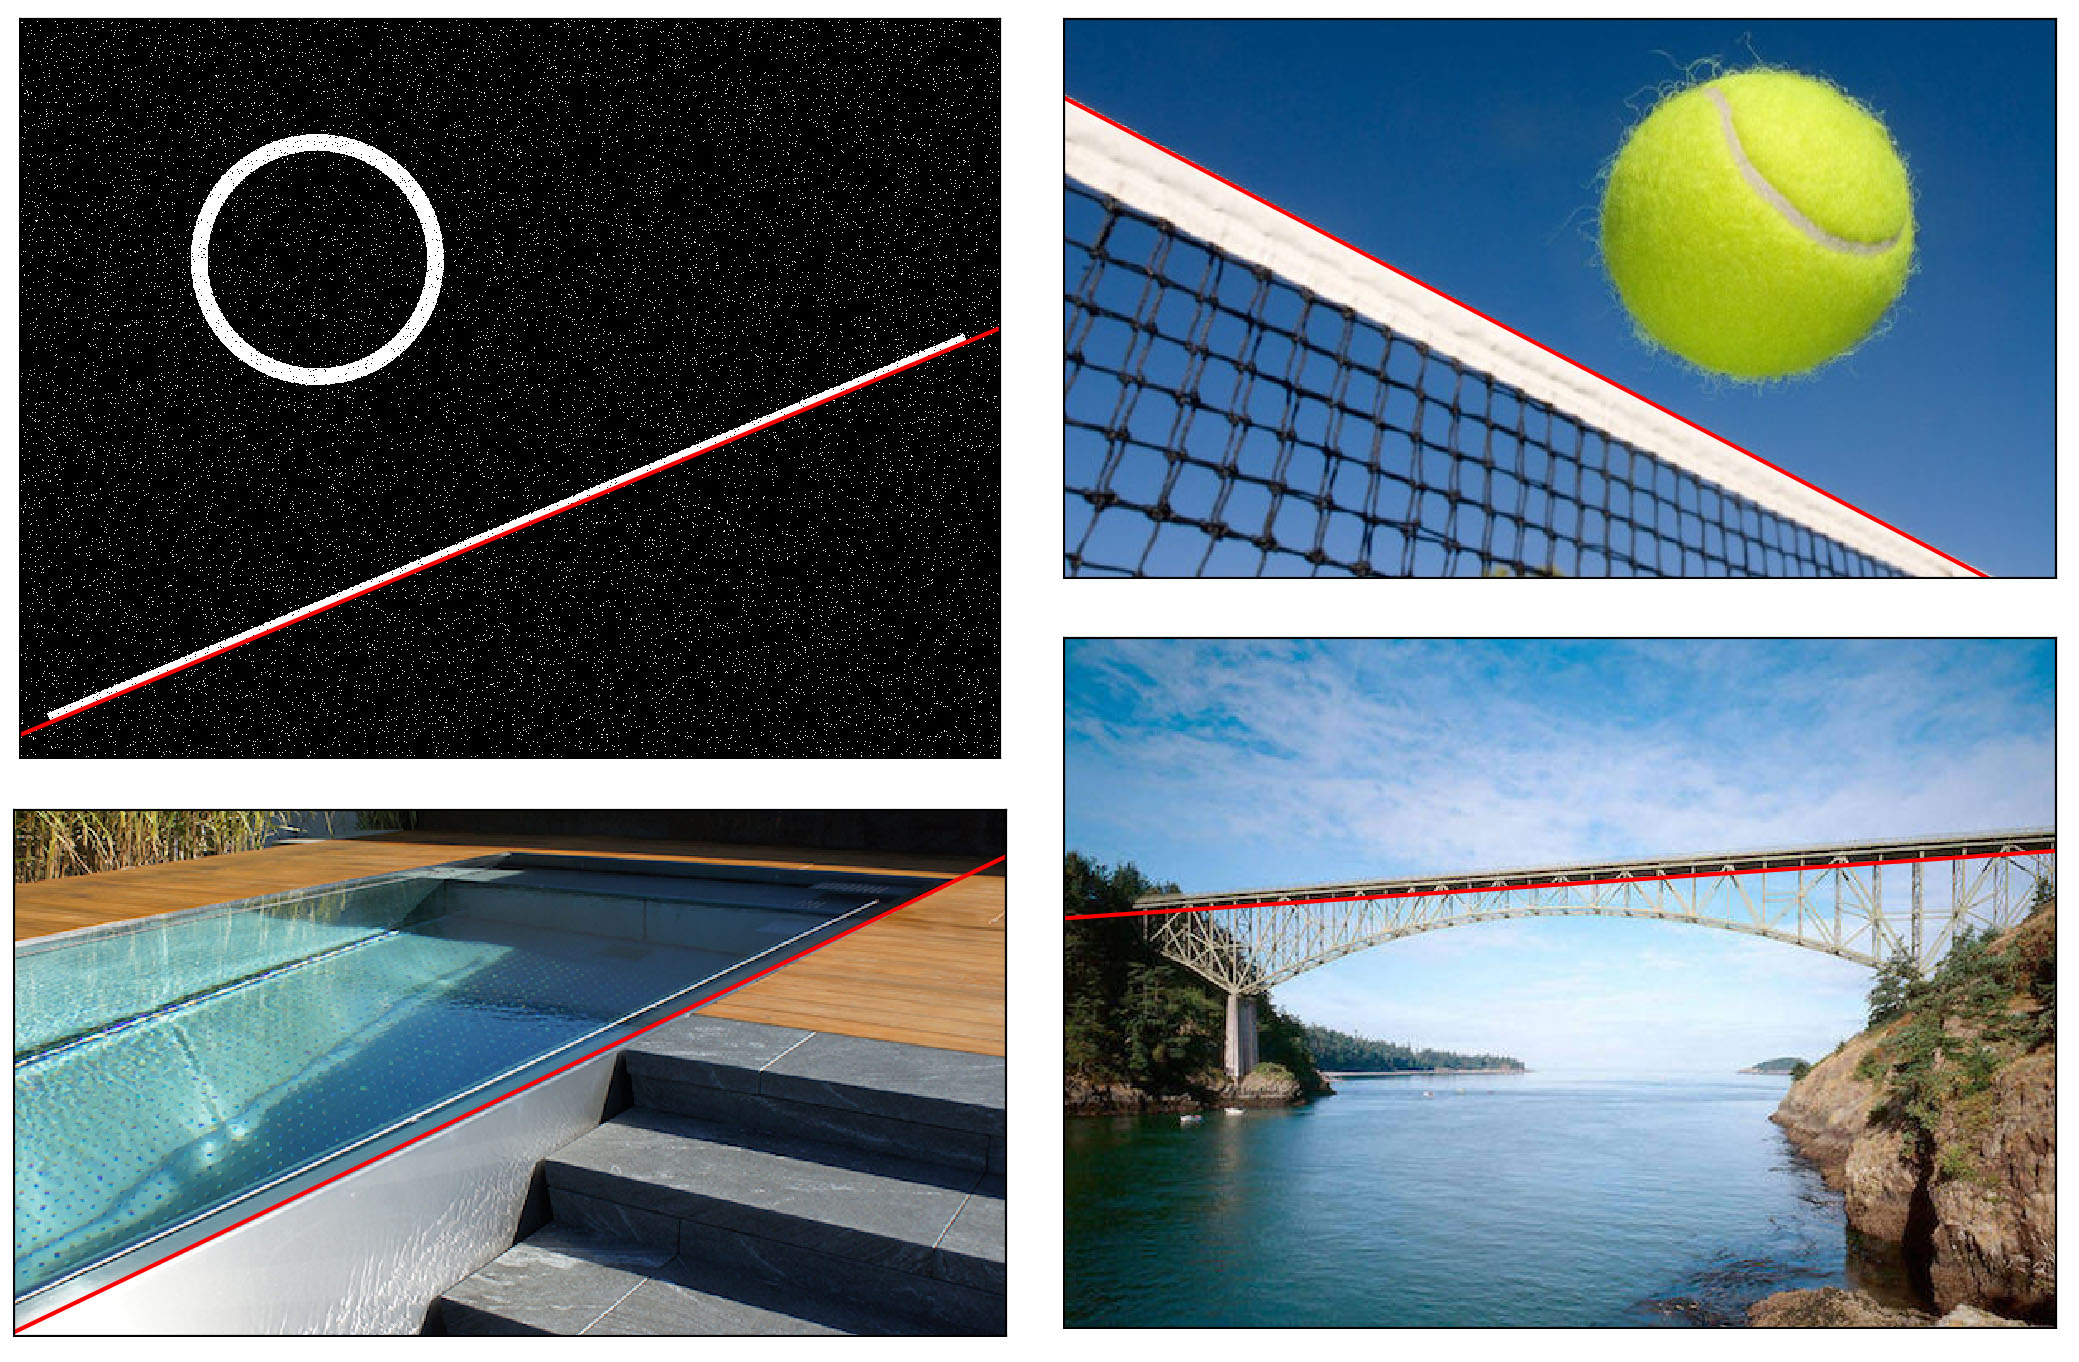
\includegraphics[width=\textwidth]{ransac_examples}
\caption{Results of correct RANSAC implementation of provided example images.}
\label{fig:ransac}
\end{figure}
  
\begin{question}
\label{find_line}
Implement a function \texttt{fit\_line} that fits a line $y=mx+c$ through two given points $(x_0,y_0)$ and $(x_1,y_1)$.
\end{question}

\begin{question}
\label{dist_from_line}
As loss function, we use the distance of all points to the line. Implement a function \texttt{point\_to\_line\_dist} that computes the minimal distance between point $(x_0,y_0)$ and a line defined by $y=mx+c$.
\end{question}

\begin{question}
As a preprocessing step, implement the function \texttt{edge\_map} that computes the edge map on an image. You are allowed to use built-in functions like \texttt{skimage.feature.canny} and \texttt{skimage.color.rgb2gray}. Try different values for the smoothing parameter \texttt{sigma} (e.g., 1, 3, 5, 10, 25). Select a value appropriate for RANSAC. Justify your choice.
\end{question}

\begin{question}
  Iterate through steps~\ref{find_line} and~\ref{dist_from_line} 500 times. For each iteration, the 2 points from which the line is generated are chosen randomly among all possible points on the edge map. The script then chooses the best fitting line and plots it on the image. As a sanity check, run your RANSAC algorithm on sample image \texttt{synthetic.jpg}. Plot and comment your results.
\end{question}

\begin{question}
  Run your script with sample images \texttt{bridge.jpg}, \texttt{pool.jpg} and \texttt{tennis.jpg}. Plot and comment your results.
\end{question}

\section{Texture Synthesis [4 points]}

In this exercise, you will implement a simplified version of the texture synthesis approach of Efros and Leung
\footnote{This technique of copying a whole patch is much faster than the center pixel as suggested in~\cite{efros99}. We are also omitting Gaussian weighted windowing. The results are therefore of inferior quality.}. 
Template code \texttt{hw3\_ex2\_template.py} and sample images are provided.

To each image corresponds a \texttt{*\_fill.jpg} and a \texttt{*\_texture.jpg} image.
These images are binary masks corresponding to the regions to fill (also refered to as masked region) and the regions where the texture will be sampled from, respectively.
Your script will produce a figure similar to fig. \ref{fig:donkey}.

\begin{figure}[h]
\centering
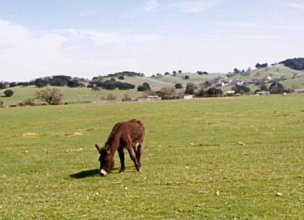
\includegraphics[width=.31\textwidth]{donkey}
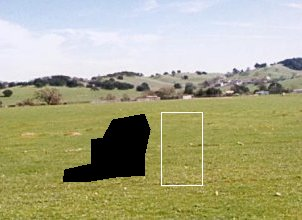
\includegraphics[width=.31\textwidth]{donkey2}
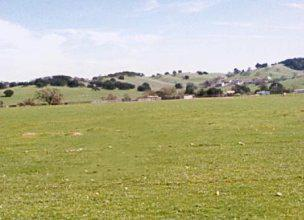
\includegraphics[width=.31\textwidth]{donkey3}
\caption{Left: original image  \texttt{donkey.jpg}. Middle: image with region to be filled (black region) and sample texture region (white rectangle). Right: resulting image you will get at the end of this exercise.}
\label{fig:donkey}
\end{figure}

The general idea of the algorithm is given here:
\begin{itemize}
  \item Randomly select a point $\bm{r}$ on the boundary of the masked region.
  \item Let $P_{\bm{r}}$ a patch centered on $\bm{r}$ of size $W \times W$. Find another patch $Q_{\bm{r}'}$, of equal size, centered on $\bm{r}'$, in the texture region, such that a dissimilarity measure $d(P_{\bm{r}},Q_{\bm{r}'})$ is minimized.
  \item Let $P_{masked, \bm{r}}$ the set of pixels in $P_{\bm{r}}$ that are masked.
    Replace each pixel $P_{masked, \bm{r}}(i, j)$  with pixel  $Q_{\bm{r}'}(i, j)$. With $(i, j) \in [0, W]^2$
  \item Repeat until there are no more masked pixels.
\end{itemize}

To do that, you may follow these steps:
\begin{question}
Write a function \texttt{compute\_ssd} that computes the Sum of Squared Difference (SSD) between a patch and a texture region, for each possible location of the patch within the texture region. It will ignore the masked pixels of \texttt{*\_fill.jpg}. Please note that:
\begin{itemize}
\item \texttt{patch}, has size \texttt{[2 * patch\_half\_size + 1, 2 * patch\_half\_size + 1, 3]}.
\item The texture region \texttt{texture}, has size \texttt{[tex\_rows, tex\_cols, 3]}.
\item \texttt{mask} specifies which elements in \texttt{patch} will be filled in. It contains a 1 for each masked pixel. Its width and height are the same as \texttt{patch}. When computing the result, ignore the masked pixels. 
\item The output array \texttt{ssd}, is of size \texttt{[tex\_rows - 2 * patch\_half\_width, tex\_cols - 2 * patch\_half\_width]}, i.e. it is only defined where the patch completely overlaps the texture. 
\end{itemize}
\end{question}

\begin{question}
  We now take the SSD image created above and chose the best match.
  This best match will be used to replace values in the masked region.
  Write a function \texttt{copy\_patch} which copies this selected patch into the final image at the appropriate location.
Replace pixel values only in the masked region of the image, i.e. unmasked pixels should be left as is.
\end{question}

\begin{question}
Plot the image after texture synthesis. The original image, the masked image, and the sample texture region, as in fig. \ref{fig:donkey}). Apply your texture synthesis script to \texttt{yacht.jpg} and \texttt{tomato.jpg}. Show your results and give a short analysis.
\end{question}

\bibliography{refs}

\end{document}